\section{Exercise ten}

A system is composed of components arranged in the following reliability block diagram:
\begin{figure}[H]
    \centering
    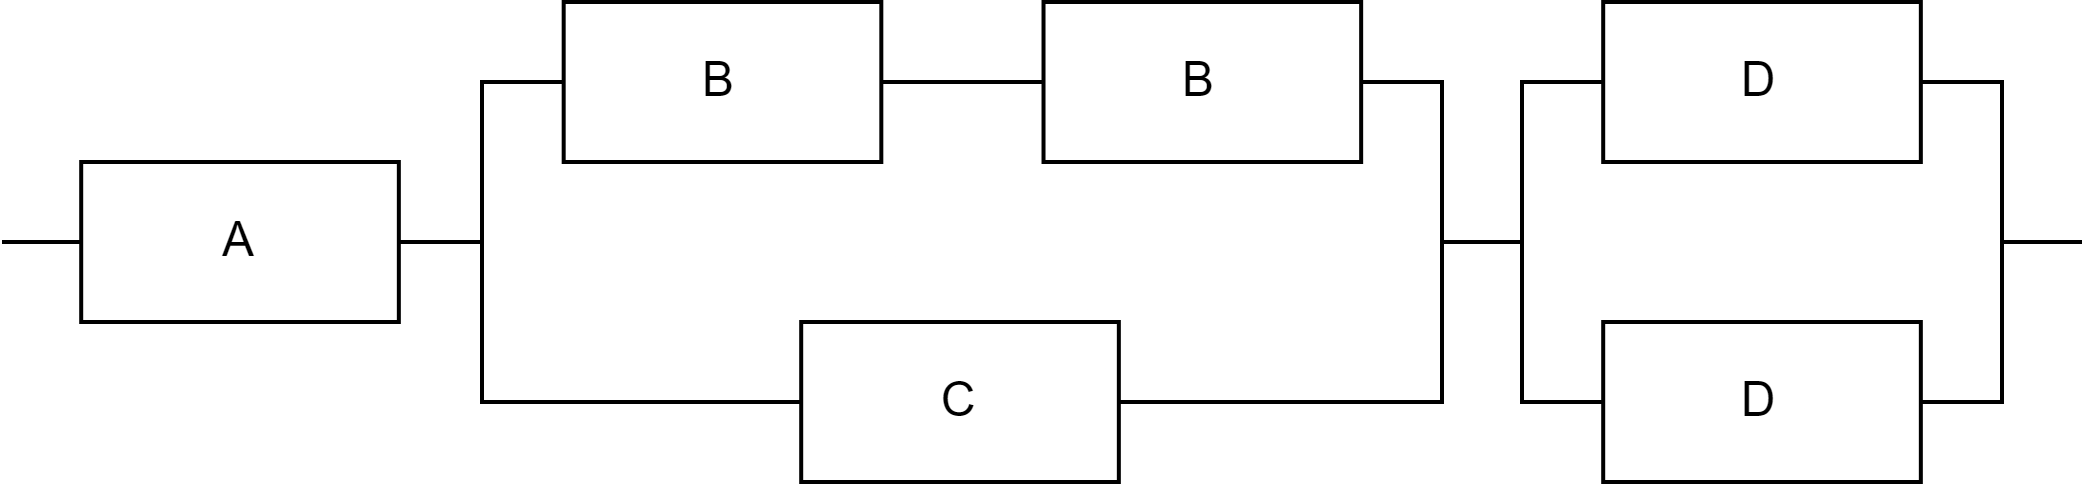
\includegraphics[width=0.7\linewidth]{images/rbd2.png}
\end{figure}
\begin{enumerate}
    \item Identify all possible configurations of components that may fail without causing the entire system to fail.
    \item Calculate $\text{MTTF}_\text{B}$ knowing that $R(t) = 83\%$ at two years.
    \item Compute the availability of the entire system given that $\text{MTTF}_\text{A}=\text{MTTF}_\text{D}=1$ year, $\text{MTTF}_\text{C} = 14$ months, and $\text{MTTR}=21$ days for all components.
\end{enumerate}

\subsection*{Solution}
\begin{enumerate}
    \item Renaming the blocks in the reliability block diagram as:
        \begin{figure}[H]
            \centering
            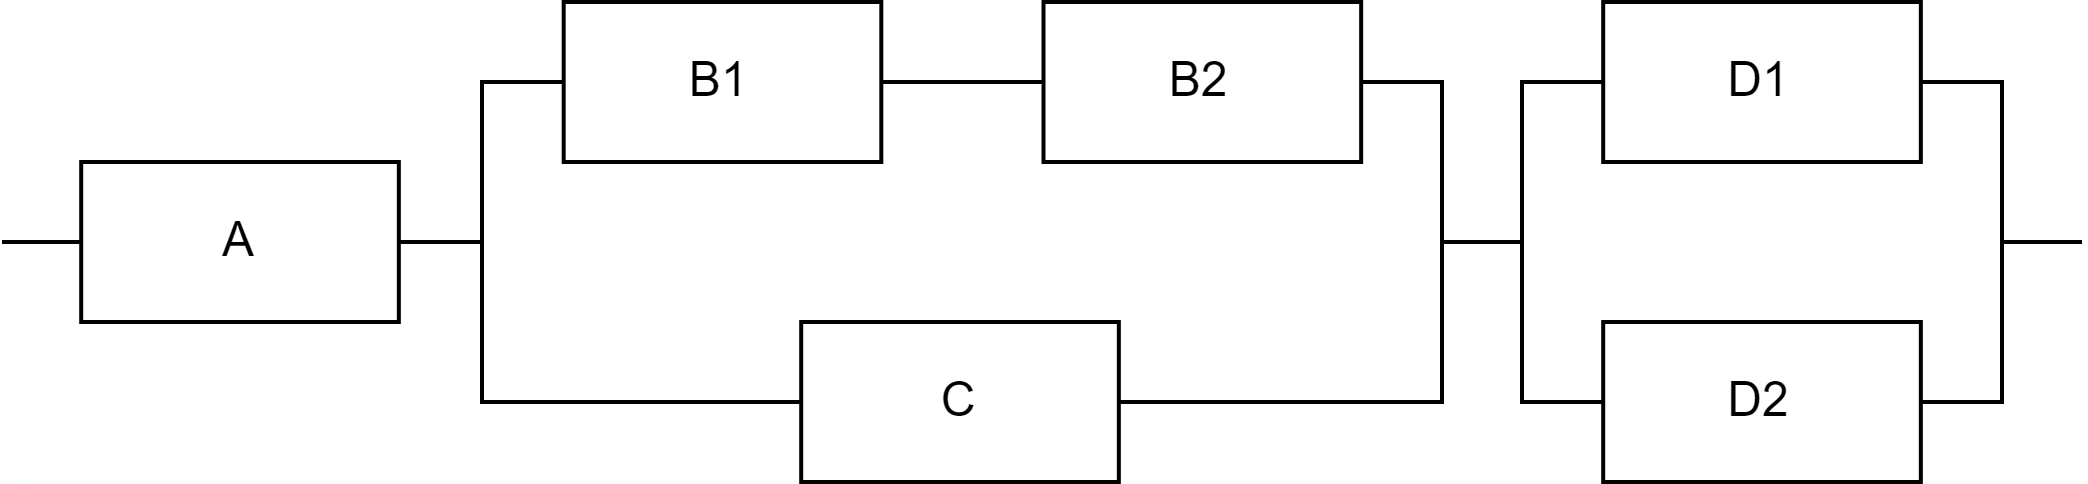
\includegraphics[width=0.7\linewidth]{images/rbd3.png}
        \end{figure}
        The pairs of blocks that may fail without causing the entire system to fail are:
        \begin{itemize}
            \item B1 and D1. 
            \item B1 and D2.
            \item B2 and D1. 
            \item B2 and D2.
            \item C and D1. 
            \item C and D2.
        \end{itemize}
    \item The reliability of each block B is calculated as:
        \[R_B(2 \text{ years})=e^{-\frac{2}{\text{MTTF}_{\text{B}}}}\]
        Given this expression equals $0.83$, we solve for MTTF:
        \[e^{-\frac{2}{\text{MTTF}_{\text{B}}}}=0.83 \rightarrow \text{MTTF}=-\dfrac{2}{\ln(0.83)}=10.73 \text{ years}\]
    \item The mean time to failure of block C in years is:
        \[\text{MTTF}_{\text{C}}=\dfrac{14 \text{ months}}{12 \text{ months}}=1.17 \text{ years}\]
        Similarly, the mean time to recovery is:
        \[\text{MTTR}=\dfrac{21 \text{ days}}{365 \text{ days}}=0.058 \text{ years}\]
        
        We can compute the availability for each block:
        \begin{itemize}
            \item $A_{\text{A}}=A_{\text{D}}=\frac{\text{MTTF}}{\text{MTTF}+\text{MTTR}}=\frac{1}{1+0.058}=0.95$
            \item $A_{\text{C}}=\frac{\text{MTTF}}{\text{MTTF}+\text{MTTR}}=\frac{1.17}{1.17+0.058}=0.95$
            \item $A_{\text{B}}=\frac{\text{MTTF}}{\text{MTTF}+\text{MTTR}}=\frac{10.73}{10.73+0.058}=0.99$
        \end{itemize}
        Now, we combine the two blocks B into a single block:
        \[A_{\text{BB}}=A_{\text{B}}A_{\text{B}}=0.99\cdot 0.99=0.98\]
        Then, we have the parallel connection between the new block and C:
        \[A_{\text{BBC}}=1-\left(1-A_{\text{BB}}\right)\left(1-A_{\text{C}}\right)=1-(0.02)(0.05)=0.999\]
        Similarly, for the parallel connection between the two blocks D:
        \[A_{\text{DD}}=1-\left(1-A_{\text{D}}\right)\left(1-A_{\text{D}}\right)=1-(0.05)(0.05)=0.997\]
        Finally, the total availability of the system can be computed as the series of A, BBC, and DD:
        \[A_{s}=1-\left(1-A_{\text{A}}\right)\left(1-A_{\text{BBC}}\right)\left(1-A_{\text{DD}}\right)=1-(0.05)(0.001)(0.003)=0.946\]
\end{enumerate}